%----------------------------------------------------------------------------------------
%	CHAPTER - DEVELOPMENT
%----------------------------------------------------------------------------------------

\chapter{Development}

\label{ChapterDevelopment}

%----------------------------------------------------------------------------------------
%	SECTION 1
%----------------------------------------------------------------------------------------

\section{Introduction}

The \textit{Development} phase, as defined by \cite{Vaishnavi2008} and \cite{Hevner2010}, comes after the \textit{Suggestion} of a design and focuses on the further development and implementation of the design. The outcome of this chapter is the requirement for the subsequent \textit{Evaluation} chapter. This is a crucial step in answering \gls{srq} 4 since the to be achieved benefits over the traditional approaches have only been of theoretical nature so far, but are not tested for their feasibility yet. \cite{Vaishnavi2008} see different techniques on how the implementation can look like, depending on the to be constructed artifact. For this thesis, the development of a prototype application in \gls{vr} has been chosen. In a first step, the technical setup is defined, before the architecture and data model for the prototype are discussed. Following that, the actual implementation of the different views and navigations are covered with a conclusion at the end. \newline
Building up on this, the \textit{Evaluation} phase will then be discussed in chapter \ref{ChapterEvaluation}.


%----------------------------------------------------------------------------------------
%	SECTION 2
%----------------------------------------------------------------------------------------

\section{Technical Setup}

The technical setup chapter gives a description and explanation for the selection of the individual components that are used for the development of the prototype application. It can be distinguished between Hardware and Software components that are discussed in their respective sub-chapters.


%-----------------------------------
%	SUBSECTION 1
%-----------------------------------
\subsection{Hardware}

The in the literature review discussed different methods for user input as part of \gls{srq} 2 have been summarized in table \ref{tbl:methodscomparison}. For the selection of the right \gls{vr} device, this conclusion was considered for the evaluation. While for the \textit{Travel} aspect only three methods (including the option for no travel at all) have been discussed:

\textbf{No travelling option:}
By looking at \gls{mdg} 2 that defines the user to be part of the \gls{ve} and thus is able to 'travel' around the visualisations, the third option would violate this design goal and thus is no viable option.

\textbf{Full Body Tracking:}
While it allows for free movement within \gls{ve}, it is lacking accuracy and only works from one angle. This can be effectively used if a static display in one direction is used which updates the data that it displays. With an implementation of the 'multiples linked views' concept however, one angle will not be enough anymore.

\textbf{360° Motion Tracking:}
Compared to 'Full Body Tracking', the '360° Motion Tracking' provides much better accuracy and allows for spatial positioning in all three axis, which strongly supports \gls{mdg} 2.


This leads to a first conclusion for '360° Motion Tracking' which is the only methods for \textit{Travel} that fulfils all requirements of the design goals. For \textit{Selection} (and \textit{Manipulation}), some more methods had been discussed:

\textbf{No selection/manipulation option:}
The option for no input method cannot be considered as the application would then provide no interaction at all and thus violate \gls{mdg} 1 that requires a high interactivity with tightly coupled actions/reactions.

\textbf{Hand Gestures:}
While 'Hand Gestures' offer a very high familiarity, they have a limited tracking area and become less accurate with faster movements. Although the latter is not of that importance, the limited tracking area can become problematic with the different views, especially since the supporting views are placed in the centre of where the user is looking at.

\textbf{Gesture Controllers:}
TODO: tbd

\textbf{Speech Recognition:}
This methods requires a silent area and good pronunciation of one of the supported official languages, as dialects can be quite problematic. While it allows for some very interesting, more complex queries such as "Show me all transactions in the last seven days over CHF 100.", it rather can be seen as a supportive input method, but not as the main input method.

\textbf{Physical Placement of Objects:}
While the 'Physical Placement of Objects' would be the most realistic and immersive option, it can be considered as to expensive and also too difficult to build as for this design goal not only some buttons and knobs would need to be built, but also fully dynamic charts and tables.


It can be concluded, that the 'Gesture Controllers' have the highest fit, and also work very well together with the '360° Motion Tracking'. Speech Recognition can provide some interesting support-functionalities that should be looked at in future research. \newline
This combination of input methods are best met with the HTC Vive (\url{https://www.vive.com/}) that was unveiled by HTC in early 2016. The bundle consists of a \gls{hmd}, two gesture controllers (as explained in Chapter \ref{SubSubSectionGestureControllers}) and two so called 'Lighthouses' (as explained in Chapter \ref{360MotionTracking}) that when set up in opposite corner allow for a full motion tracking.



%-----------------------------------
%	SUBSECTION 2
%-----------------------------------

\subsection{Software}

All used software for the development of the \gls{vr} prototype is summarised and described in the following sub-chapters.


\subsubsection{Game Engine}
At the foundation, \cite{Unity2016} multi-platform game engine and development toolkit 'Unity 3D' is used. It offers the option to not only develop 2D applications, but also 3D applications that can be run in \gls{vr}. It is used for the actual design of the \gls{ve} and the configuration of 3D objects.

\textbf{Software:} Unity 3D \newline
\textbf{Version:} 5.5.0f3 \newline
\textbf{Link:} \url{http://unity3d.com/}


\subsubsection{Game Engine Plugins}
For the integration of the \gls{sdk} to access the specific methods and functions of the HTC Vive, the SteamVR plugin for Unity is used \citep{Valve2016a}. In addition to this, \gls{vrtk} will be used as a toolkit to rely on 'standardised' ways for certain \gls{vr}-specific interactions and functions in Unity 3D \citep{Sysdia2017}. Even though the HTC Vive has been chosen for the hardware part, due to the usage of the SteamVR plugin and the \gls{vrtk}, only little to none changes should be required in order to have the prototype application also run other supported hardware such as the Oculus Rift, since both of them support multiple \glspl{hmd}.

\textbf{Software:} SteamVR Plugin \newline
\textbf{Version:} 1.1.1 \newline
\textbf{Link:} \url{https://www.assetstore.unity3d.com/en/#!/content/32647}

\textbf{Software:} \gls{vrtk} - Virtual Reality Toolkit \newline
\textbf{Version:} 3.0.0 \newline
\textbf{Link:} \url{https://www.assetstore.unity3d.com/en/#!/content/64131} \newline
\textbf{Link:} \url{https://vrtoolkit.readme.io/}


\subsubsection{\gls{ide}}
Visual Studio Community 2015 from \cite{Microsoft2015} is used for the development of the Unity Scripts in the programming language C\#. These scripts handle and manage the whole \gls{ve} by triggering interactions of the 3D objects defined and placed in Unity 3D.

\textbf{Software:} Microsoft Visual Studio Community \newline
\textbf{Version:} 2015 \newline
\textbf{Link:} \url{https://www.microsoft.com/en-us/download/details.aspx?id=48146}
 

\subsubsection{3D Graphics}

Finally, for the design of custom 3D models as representations of the category icons as shown in Figure \ref{fig:categoriesicons} in Chapter \ref{SubSectionCategoriesFiltering}, the  open-source 3D computer graphics software Blender is used \citep{Blender2016}. The exported models are fully compatible with Unity 3D and can be seamlessly imported and used.

\textbf{Software:} Blender \newline
\textbf{Version:} 2.78a \newline
\textbf{Link:} \url{https://www.blender.org/}




% USE ONLY IF REMOVED FROM CHAPTER 1 (DELINEATIONS ETC)
%\begin{figure}[h]
%	\begin{center}
%		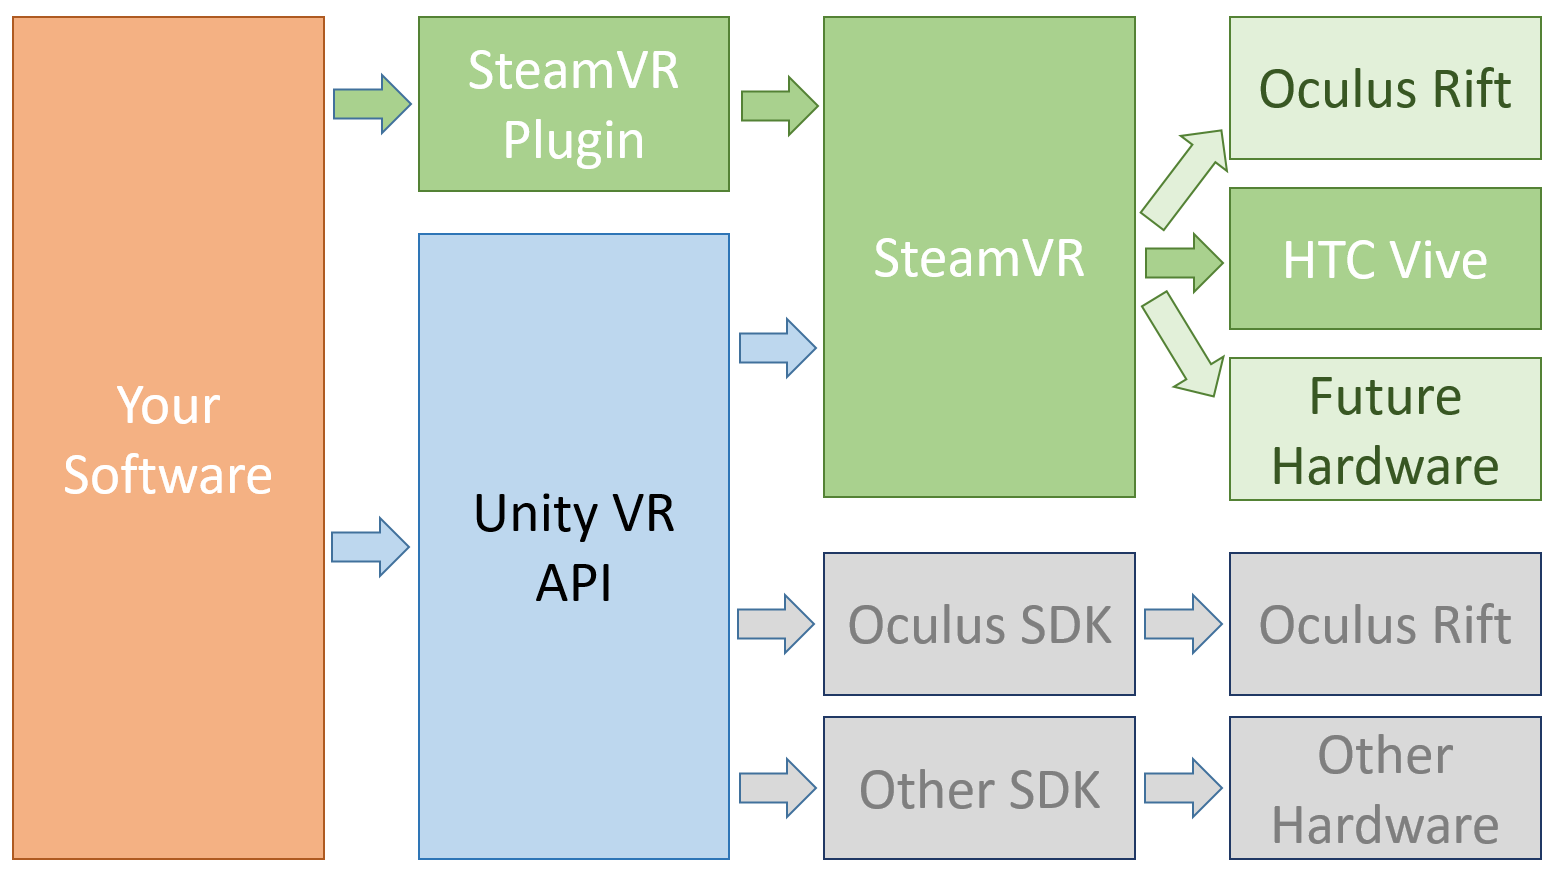
\includegraphics[width=14cm]{03_Figures/04_Valve/OpenVR_SteamVR_selected.png}
%		\caption[Steam VR Unity Plugin]{Steam VR Unity Plugin (adopted from \cite{Valve2016})}
%		\label{fig:steamvrselected}
%	\end{center}
%\end{figure}



%----------------------------------------------------------------------------------------
%	SECTION 3
%----------------------------------------------------------------------------------------

\section{Architecture}

TODO:
3. architecture





%-----------------------------------
%	SUBSECTION 1
%-----------------------------------
\subsection{Subsection 1}

tbd


%-----------------------------------
%	SUBSECTION 2
%-----------------------------------

\subsection{Subsection 2}

tbd


%----------------------------------------------------------------------------------------
%	SECTION 4
%----------------------------------------------------------------------------------------

\section{Data Model}


TODO:
4. data model



%----------------------------------------------------------------------------------------
%	SECTION 5
%----------------------------------------------------------------------------------------

\section{Implementation of Views and Navigation}


TODO:
5. implementation of views and navigation
- Code Structure?
- (Unity) Object Design
- (Unity) Script Design
- Important Code Snippets?
- Screenshots



Category Selection - waiting for data load --> coloring!
\gls{mdg} 1 that requires a high interactivity with tightly coupled actions/reactions.


%----------------------------------------------------------------------------------------
%	SECTION 6
%----------------------------------------------------------------------------------------

\section{Conclusion}


TODO:
6. Conclusion



%% IDEA FOR PROTOTYPE

% - Start with a small table on which a house etc is visualized. floating above is year (+month)
% + Each object represents one category from the financial expenses.
% - maybe size indicates the overall amount?
% - The colours depends on the difference between my planned expenses (or average expenses) and the actual expenses. less = green, about the same = yellow-(green-)ish, slightly above = orange, above = red.
% - By clicking on one of the objects, it gets highlighted and a line-chart appears showing the expenses
% A) show individual transactions for the given month up until the threshold
% B) show individual months until the threshold (+forecast?)
% - show multiple lines for the different sub-categories (enable/disable) plus the total
% - clicking on an entry of the line chart displays details about transaction (amount, location), or the month (amount) in an overlay
% - switching between single-month and year view by... using the touchpad (up/down clicks)
% - navigating through months/years by... a using the touchpad! (left/right clicks)
% - resetting the view to start by... clicking on the select button

% - maybe outside as rotating rings: the individual bank accounts?
